\section{Lösungsansatz}

Zur Berechnung größerer Graphen gibt es sogenannten metaheuristische Verfahren die keine optimale Lösung garantieren.
Durch probabilistische Schätzungen und heuristische Verfahren können jedoch gute Lösungen gefunden werden.
\\\\
Eines dieser metaheuristischen Verfahren ist der Ant Algorithm (auch \glqq Ant Colony Optimization\grqq{} oder \glqq \acs{aco}\grqq{} genannt).
Dies ist ein Algorithmus der sich an dem Verhalten von Schwärmen von Tieren orientiert.
Ein Schwarm besteht aus einer Gruppe von \glqq Agenten\grqq{} die miteinander kommunizieren, um eine Lösung zu finden.
Der \acs{aco} basiert auf dem Verhalten von Ameisen, die Pfade zu Nahrungsquellen aufspüren.
\\
Der Algorithmus simuliert die Aktivitäten von Ameisen, die zufällig durch die Städte wandern und dabei Informationen über die Qualität der verschiedenen möglichen Pfade sammeln.
Bei jeder Bewegung einer Ameise werden auf dem gewählten Pfad Pheromone (Duftstoffe) hinterlassen.
Diese Informationen werden dann verwendet, um die Wahrscheinlichkeit zu bestimmen, dass eine bestimmte Ameise einen bestimmten Pfad wählt, wenn sie von einer Stadt zu einer anderen reist.
\\
Zur weiteren Optimierung der Tour werden nacheinander mehrere Generationen von Schwärmen durchlaufen.
Jede Generation bekommt die Wahrscheinlichkeiten der Pfade der vorherigen Generation und baut darauf auf.
Auf diese Weise kann der Algorithmus schrittweise die optimale Tour durch die Städte bestimmen.

\begin{figure}[h]
    \centering
    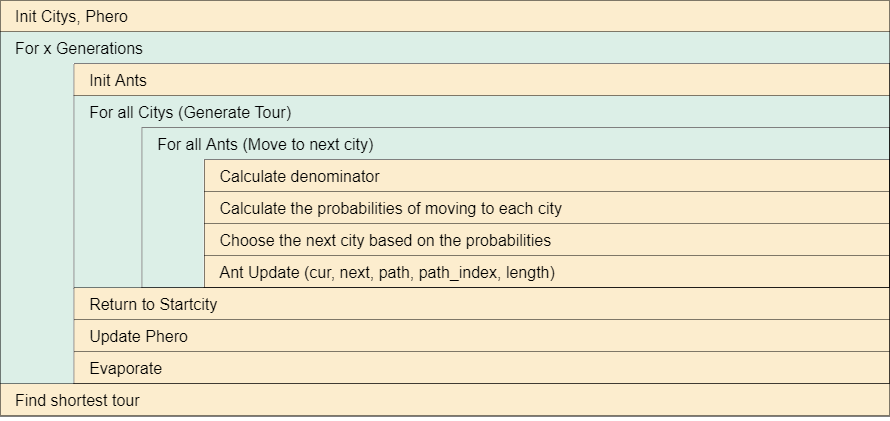
\includegraphics[width=16cm]{../images/struktog.png}
    \caption{Algorithmus Struktogramm}
    \label{fig:struktogramm}
\end{figure}

\section{Implementierung inklusive Schwierigkeiten}
1 - 2 Seiten\\
\subsection*{C Implementierung}

Damit die Verfahren vergleichbar sind, brauchen wir immer gleiche Ausgangsdaten und können diese daher nicht generieren, sondern laden diese über CSV Dateien.
Dabei besteht jede Stadt aus zwei Koordinaten, die in den Dateien gehalten werden.
Die Distanz, zur Vereinfachung die Luftlinie, zwischen zwei Städten wird mittels der Koordinaten berechnet.
\\\\
Alle Daten zur Berechnung des Pfades sind in einem Ameisen-Struct enthalten.
Dies umfasst unter anderem den Pfad der Ameise, welche Städte sie besucht hat und die Länge der Tour.
Jene Daten werden bei jeder Generation zurückgesetzt.
Im Gegensatz dazu wird die Pheromonmatrix nicht zurückgesetzt und lässt somit die Ergebnisse der vorherigen Generationen mit einfließen.
Nach jedem Durchlauf wird die Pheromonmatrix abhängig von den berechneten Tourlängen angepasst und eine natürliche Verdunstung durchgeführt.
\\\\
Abschließend wird aus der letzten Generation die beste Tour gefunden und ausgegeben.
\\\\
Zur Bewertung des Ergebnisses haben wir folgendes \href{https://poolik.github.io/visual-aco/}{ACO-Onlinetool} verwendet.
\begin{table}[h]
    \centering
    \begin{tabular}{|l|l|}
    \hline
                    & Pfadlänge bei 400 Städten     \\ \hline
    Online ACO Tool & $\sim$13.000                  \\ \hline
    Plain C         & $\sim$13.500                  \\ \hline
    \end{tabular}
    \caption{\label{demo-table}Pfadlängenvalidierung}
\end{table}

\begin{figure}[H]
    \centering
    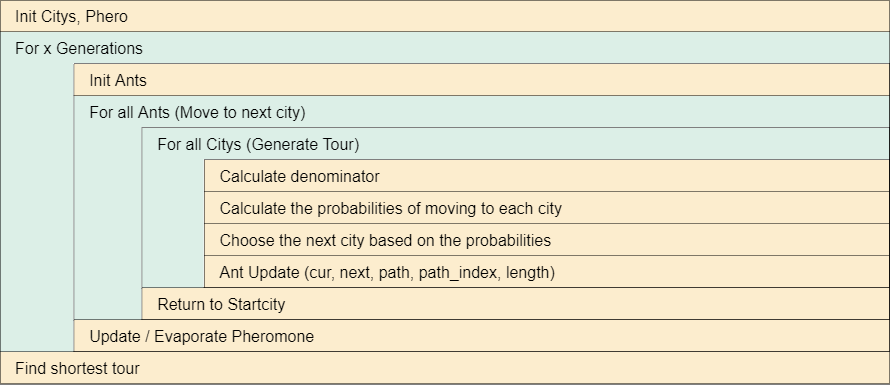
\includegraphics[width=16cm]{../images/struktog-optimiert.png}
    \caption{Algorithmus Struktogramm Optimiert}
    \label{fig:struktogramm-optimiert}
\end{figure}

\subsection*{Anpassung für OpenMP}

Es lohnt sich generell, mit OpenMP zu optimieren, wenn ein Programm eine hohe Parallelisierbarkeit aufweist, d.h. wenn es große Bereiche gibt, 
die sich gut parallel ausführen lassen und damit eine signifikante Leistungssteigerung erreicht werden kann.
Dabei ist zu beachten, dass nicht jeder Code für die Optimierung mit OpenMP geeignet ist. Speziell bei Schleifen mit geringen Iterationen und einfachen Berechnungen kann der Overhead von OpenMP die gewonnene Optimierung ausgleichen.
\\\\
Der ACO Algorithmus beinhaltet eine geschachtelte Schleife über Ameisen und Citys, in der die Berechnung der Touren stattfindet.
Innerhalb der Schleife bilden die Ameisen unabhängig voneinander ihren Pfad und müssen nicht miteinander synchronisiert werden.
Erst wenn die Generation der Ameisen durchgelaufen ist, wird die gemeinsame Pheromonmatrix aktualisiert.
Zur Pfadberstellung wird eine Wahrscheinlichkeitstabelle berechnet, welche die Wahrschienlichkeiten von der aktuellen zu jeder noch unbesuchten Stadt enthält.
Diese wird den Threads als private Variable mitgegeben, damit die Berechnungen unabhängig voneinander stattfinden können.
Somit eignet sich die innere geschachtelte Schleife aus Ameisen und Städten gut für die Optimierung mittels OpenMP.
\\\\
Weitere Schleifen welche mit OpenMP optimiert werden können sind die Aktualisierung und Verdunstung der Pheromonmatrix.
Trotz kleinem Rechenaufwand weißen sie eine hohe Anzahl an Iterationen und parallel durchführbaren Rechenschritten auf.
\\\\
Nach der letzten Ameisengeneration wird die kürzeste Tour festgestellt.
Dies geschieht innerhalb einer Schleife, die sowohl die Ameisen als auch die Städte durchläuft und dabei einen Index festlegt, der die kürzeste Tour angibt. 
Dieser Vorgang wird parallel durchgeführt, indem der Index als "Reduktion" mitzugeben wird. 
Das bedeutet, dass jeder Thread eine Kopie des Index hat und die Schleife parallel ausgeführt wird. 
Jeder Thread vergleicht die eigene Länge der Tour mit der aktuell kürzesten Tour. 
Am Ende wird nur der Index der wirklich kürzesten Tour übernommen und die anderen Kopien des Index werden verworfen.

\subsection*{Anpassungen für OpenCL}

Unser Algorithmus verwendet drei ineinander geschachtelte Schleifen, welche in die drei möglichen Dimensionen der Grafikkarte geladen werden könnten.
Um den Zugriff auf die besagten Datenfelder zu verstehen, wurde in dem Struktogramm zu jedem Schritt der Lese- (R) oder Schreibzugriff (W) notiert.
Die Grundlage für die Implementierung ist jedoch, dass passende Synchronisieren der Kernels, um die Richtigkeit des Algorithmus zu garantieren.
Die Anpassung der Pheromonematrix nach jeder Generation ist so ein Fall, wodurch eine Parallelisierung der Generationen nicht möglich ist.
Ebenso setzt der Algorithmus vorraus, dass erst die nächste Stadt berechnet werden kann, wenn die vorherige gefunden wurde.
Folglich müssen die Städte in derselben Dimension der Grafikkarte geladen werden, um die Abhängigkeit zu gewährleisten.

\begin{figure}[h]
    \centering
    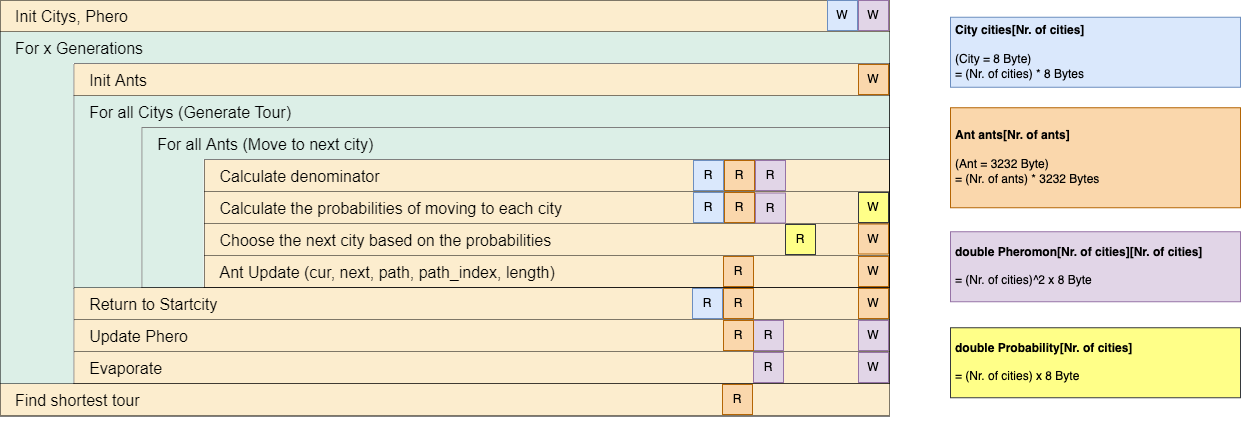
\includegraphics[width=\textwidth]{../images/Speicherzugriff.png}
    \caption{Struktogramm mit Speicherzugriff}
    \label{fig:struktogramm-speicher}
\end{figure}

Anhand des Diagramms und mit dem Ziel möglichst gleiche Speicherzugriffe zu tätigen wurde auch hier die Ameisen- und die Stadtschleife getauscht.
Das resultiert darin, dass in jedem Kernel auf die jeweils gleiche Ameise geschrieben werden kann.
Die anderen Datenfelder werden innerhalb der beiden Schleifen nur im Lesezugriff benötigt und benötigen auch keine Synchronisierung.
Zusätzlich kann das Probability Array in den lokalen Speicher des Kernels gezogen werden.
Eine zweidimensionale Berechnung der Städte bleibt jedoch weiterhin unvorteilhaft.

Ein weitere technische Hürde ist die mangelnde Unterstützung von OpenCL von zweidimensionalen Arrays, weswegen die Pheromonmatrix angepasst wurde.
Die mathematischen Methoden pow und sqrt sind in OpenCL verfügbar, jedoch kann OpenCL keine pseudozufälligen Zahlen mit rand berechnen, die aber für die Wahl der nächsten Stadt benötigt wird.
Als Ersatz wird ein Algorithmus verwendet, welcher der Implementierung von java.util.Random.nextInt() ähnelt und in den ein zufälliger Seed einfliest.
Dieser Seed wird auf dem Host für jede Generation neu berechnet und an die GPU übergeben.

Auf dem Host wurde neben dem Programmcode für OpenCL, also Vorbereitung, Speicherbefüllung / Lese und der Ausführung des Kernels noch Statements für das Benchmarking hinzugefügt.

\section{Bewertung}
Bewertung des Ansatzes und der performance-limitierenden Faktoren (1-2 Seiten)

\subsection{OpenMP}
Aufgrund der geschachtelten Schleife mit vielen Iterationen und wenig Synchronisierungen ist der Algorithmus optimal für OpenMP.
Außerdem ist der Speicher nicht so limitiert wie bei der GPU, was OpenMP einen deutlichen Vorteil verschafft.

\subsection{OpenCL}
Das größte Problem im Vergleich zur CPU ist die Menge des verfügbaren Speichers.
Dieser entspricht auf unserem Testgerät 65KB pro Workitem und global maximal 4GB.
Betrachtet man die Grafik \ref{fig:struktogramm-speicher} wird klar, dass die Pheromonmatrix schon bei 400 Städten deutlich nicht mehr in den lokalen Speicher passt.
Zudem sind hier die Zugriffe zufällig, da sie darauf basieren, in welcher Stadt sich die Ameise aktuell befindet, was zu einigen Cache Misses führen dürfte.

Die Benchmarks zeigen, dass das Ausführen des Kernels im Vergleich zu dem Lesen und Schreiben der Buffer den Großteil der Zeit in Anspruch nimmt.
Führt man den Kernel auf der CPU aus, wird die Lösung wesentlich besser und nähert sich damit an die OpenMP Lösung an.
Dieser Fakt passt zu der Theorie, dass die Speichergeschwindigkeit das Problem ist.
Eine versuchte Gegenmaßnahme kann in der Branch failed\_opt - use\_local\_phero gefunden werden, in der die Pheromonmatrix zu Beginn in den lokalen Speicher geladen wird.
Dieser Ansatz hat die Durchlaufzeit nicht verbessern können.
Vermutlich da das Übertragen ebenso Zeit benötigt und man durch den begrenzten lokalen Speicher nur noch ca. 50 Städte verwenden kann.
Dem könnte man entgegen wirken, indem die Pheromonmatrix auf float reduziert wird, was jedoch die Genauigkeit des Algorithmus verringert und so an der Vergleichbarkeit gekratzt.

Als zweiter großer Kritikpunkt ist die Generierung der Zufallszahlen zu erwähnen. 
Die generierten Zahlen wirkten bei der Entwicklung gar nicht so zufällig und die Mechanik für die Veränderung der Ganzzahl in eine Kommazahl zwischen 0 und 1 ist nicht so effizient wie in der Implementierung ohne OpenCL.

Durch die Pheromonmatrix, die an vielen Stellen bei der Berechnung benötigt wird, ist unser Algorithmus vermutlich grundsätzlich nicht gut für die GPU geignet.
Die Zufallsentscheidungen der Ameisen sorgen ebenfalls für zufällige Zugriffe, sodass man die Pheromonmatrix auch nicht in Teilen in den Kernel laden könnte.
Theoretisch müsste die OpenCL Lösung bei einer hohen Anzahl an Ameisen und einer geringen Anzahl an Städten einen Vorteil haben.

\subsection{OpenMP}

\subsection{Benchmarks}